\chapter{Adding Figures To Your Document}

\section{My First Figure}

Adding figures is easy in \LaTeX. You just create a figure environment which is much the same as the table environment. For example, put

\begin{verbatim}
\usepackage{graphicx}
\end{verbatim}
in the preamble, then put
\begin{verbatim}
\begin{figure}[!ht]
	\centering
	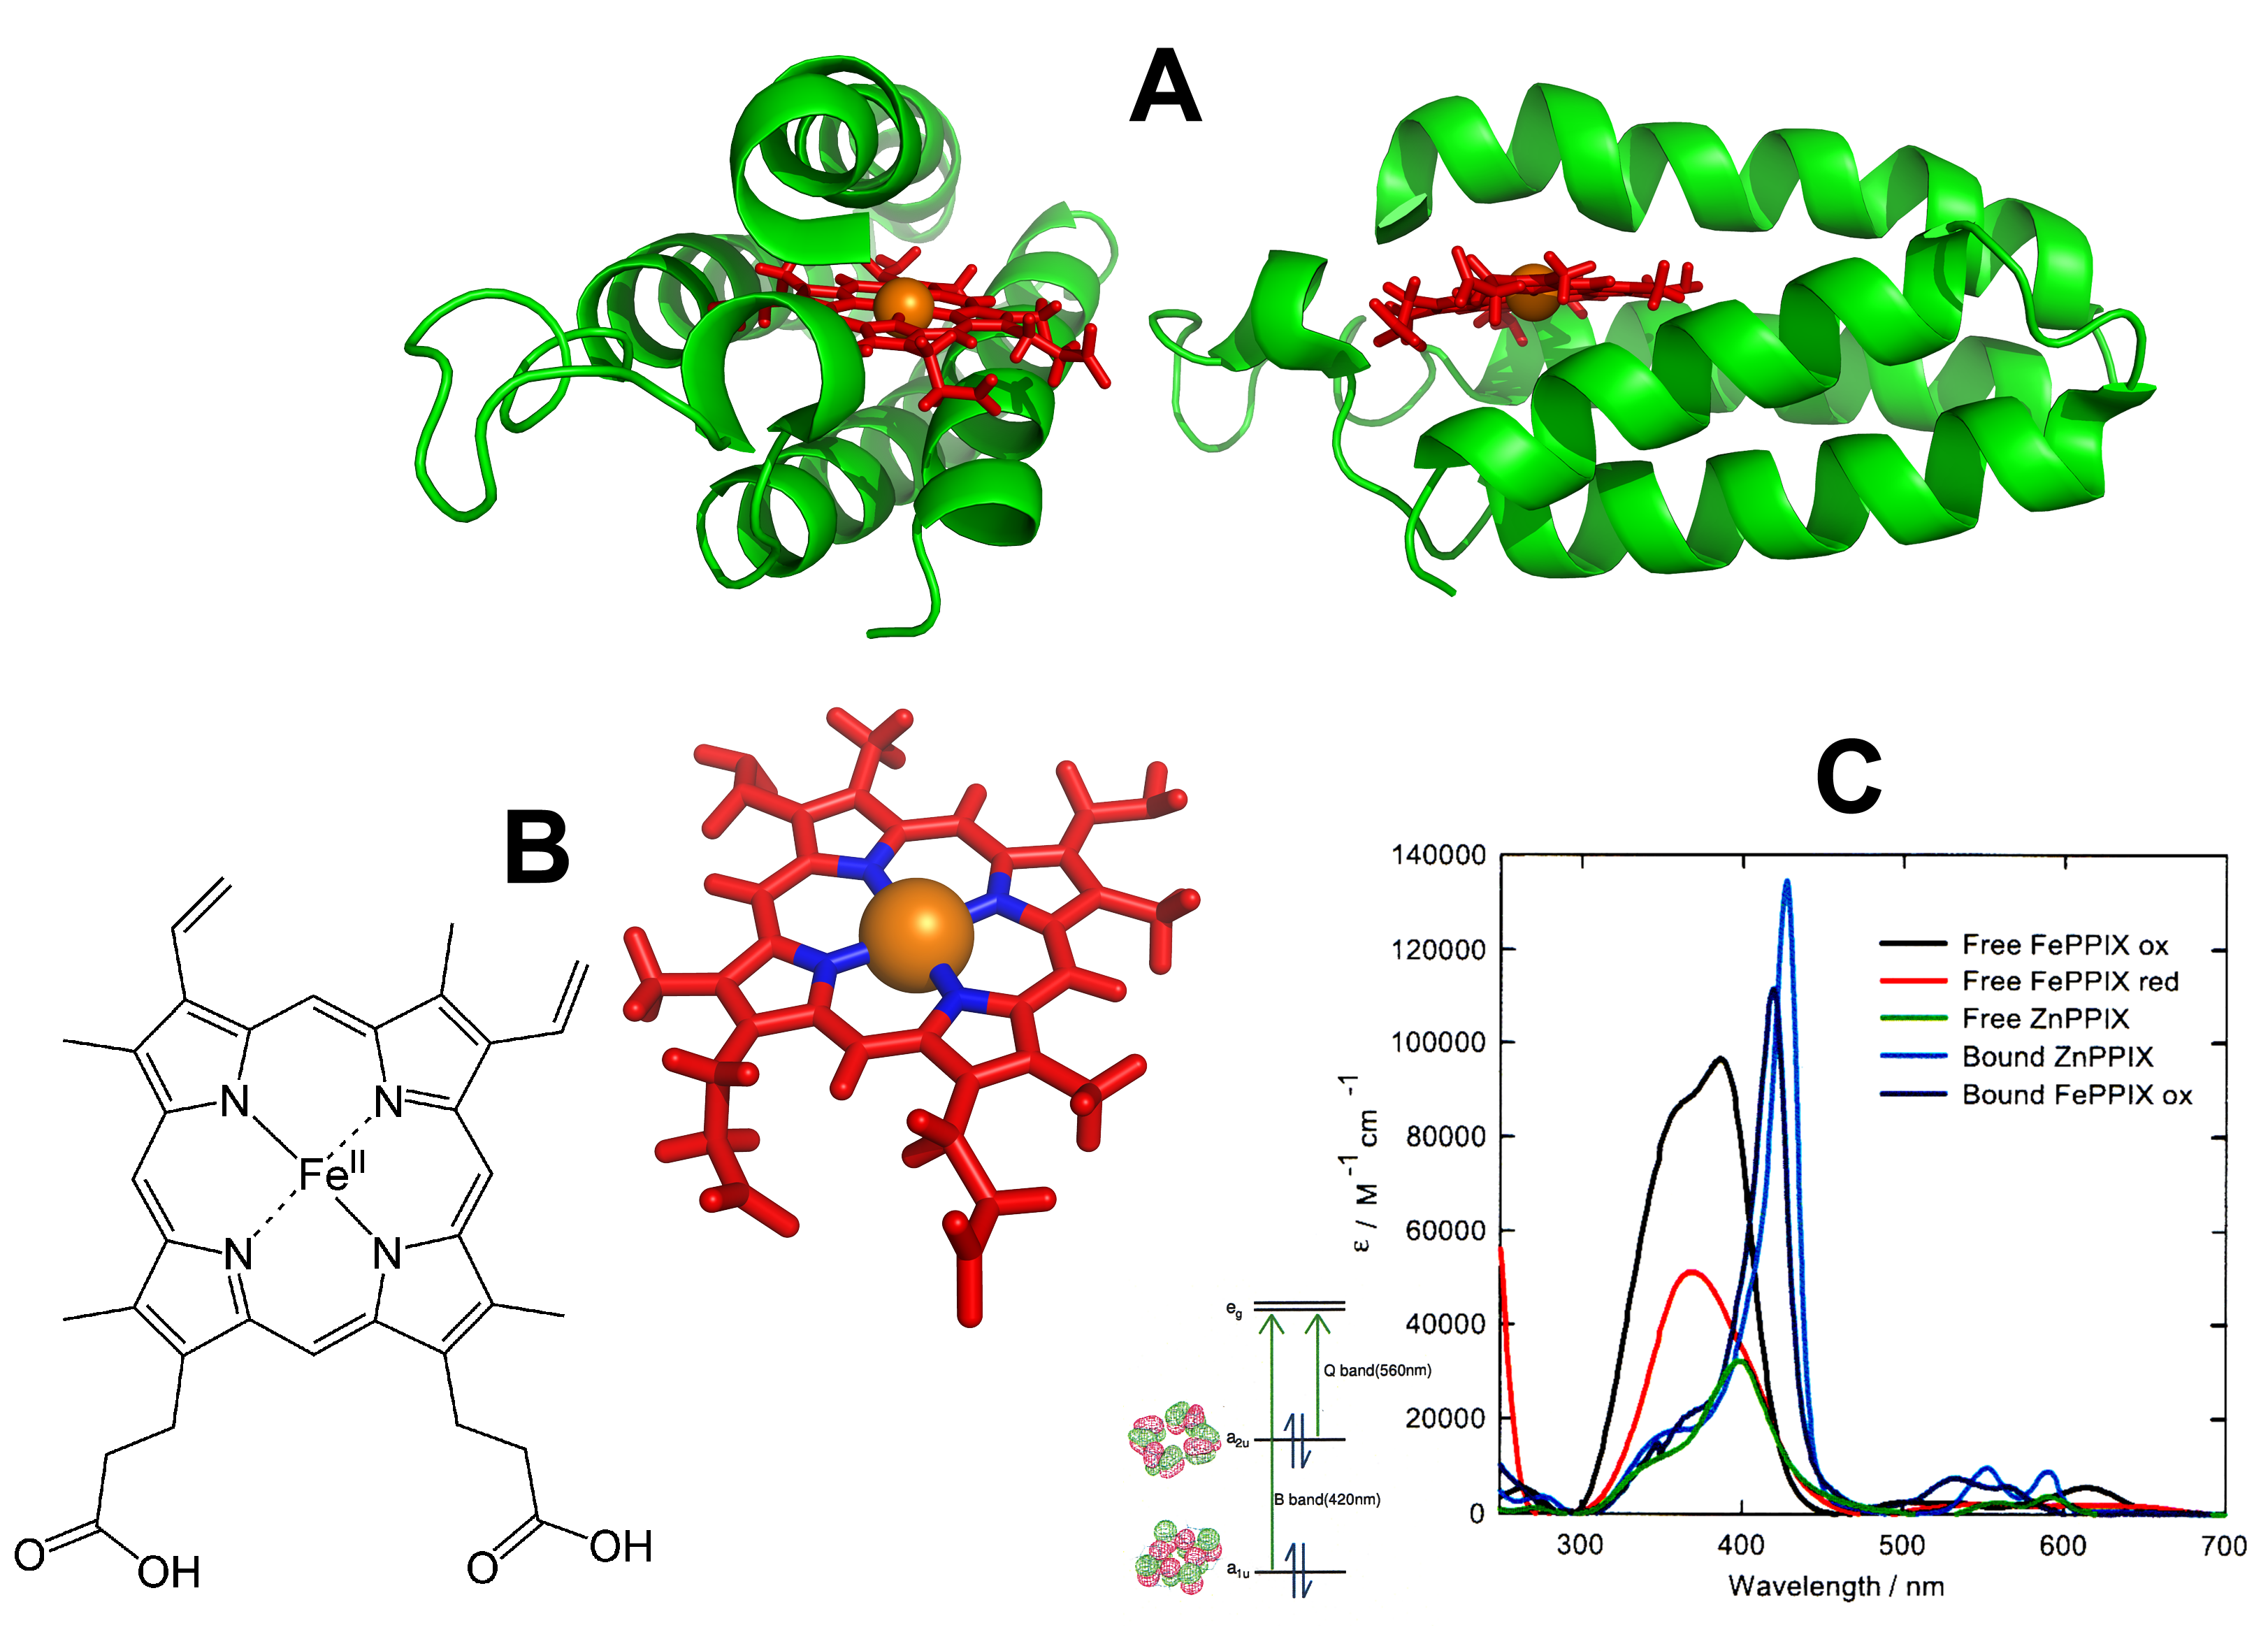
\includegraphics[width=137.4mm]{Images/haemStructure.png}
	\caption[Haem Structure]{A fancy image.}
	\label{fig:haemStructure}
\end{figure}
\end{verbatim}
in the main document, and see next page for the result. The command {\textbackslash}includegraphics tells \LaTeX\ to look in the directory ``Images'' and incorporate the file called ``haemStructure.png'' into the final document, while setting the image width to 137.4mm. This command can be used to resize a graphical file using the height or width parameter, whose value can be specified in terms of specific units (e.g.~mm, cm, pt, ex, em, and so on) or expressed as a fraction of another length parameter value (e.g.~width=0.5{\textbackslash}textwidth). \LaTeX\ recognises a very wide variety of standard units and graphics formats. The command is part of the graphicx package, and so in the preamble you must include the command {\textbackslash}usepackage\{graphicx\}.

\begin{figure}[!ht]
	\centering
	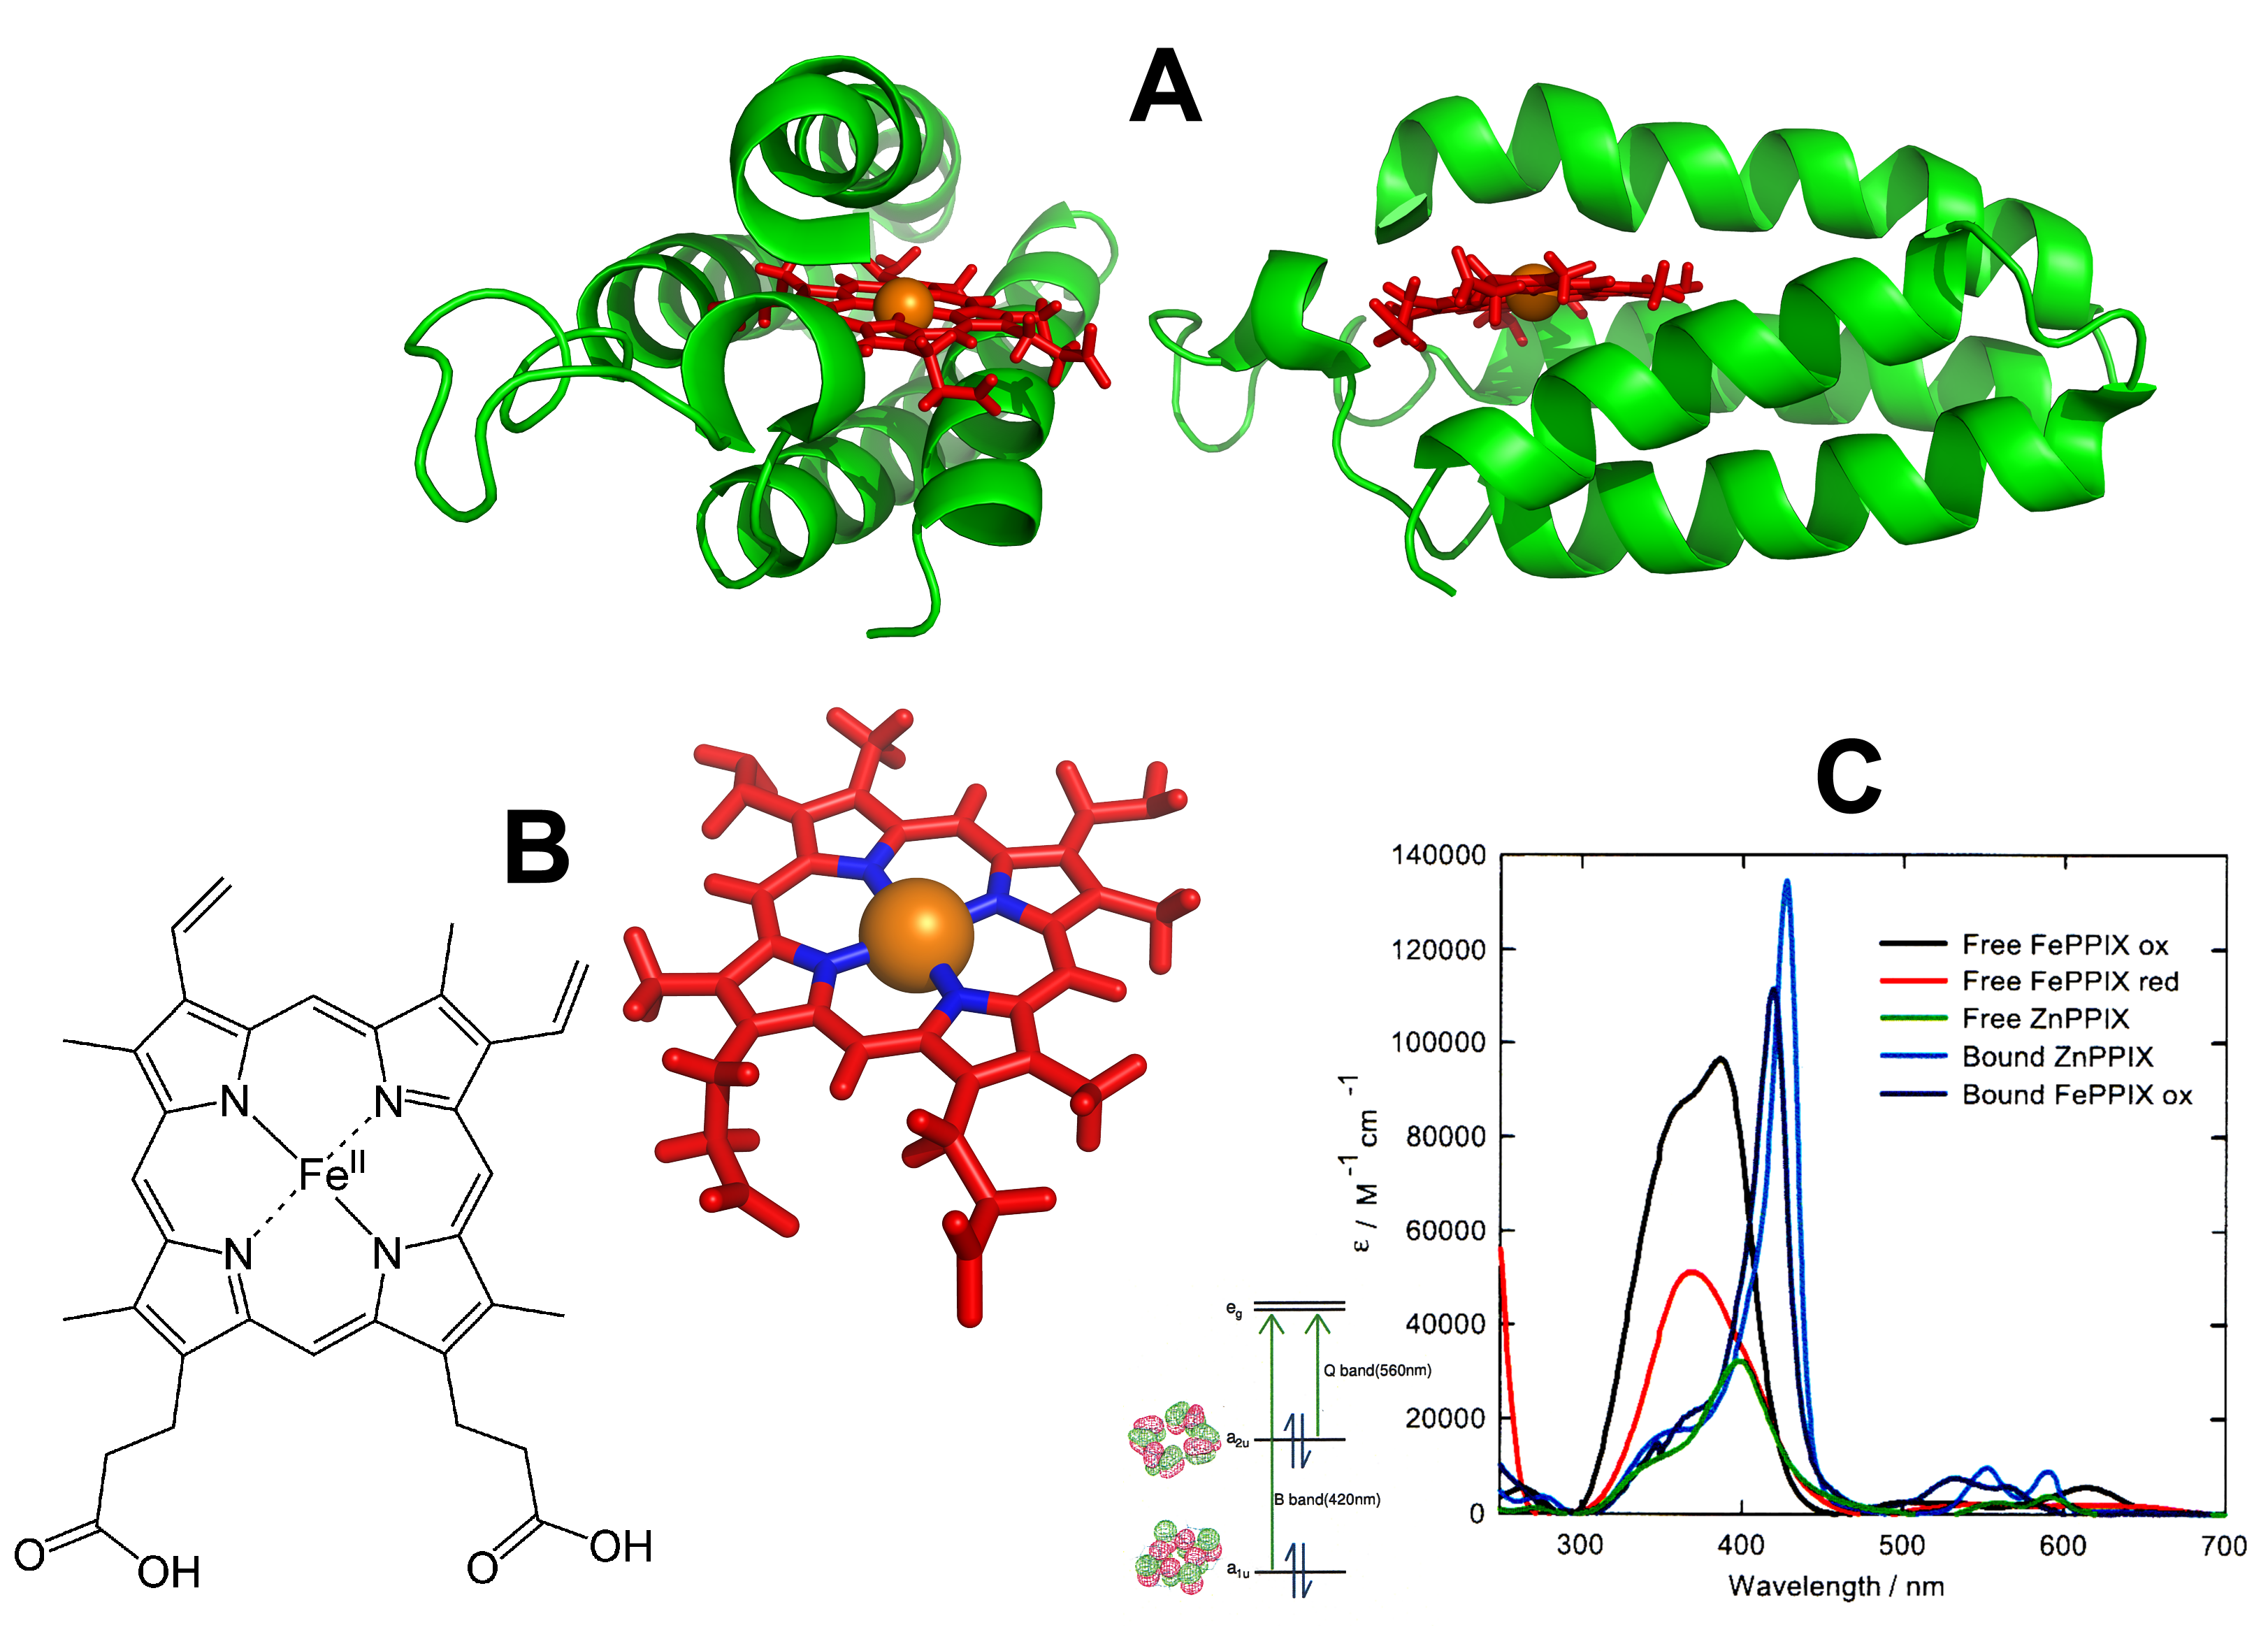
\includegraphics[width=137.4mm]{Images/haemStructure.png}
	\caption[Haem Structure]{A fancy image from Chris Forman's Thesis.}
	\label{fig:haemStructure}
\end{figure}

Many packages have been written to provide new commands. For example the `subfigure' package enables you to place separate images or files in the same figure side by side while giving them their own label. However, in this document we only concentrate on the very basics.

\section{Floating Environments}

Both tables and figures are examples of a ``floating environments'', which means \LaTeX\ decides where to put them.

The mysterious [!ht] letters give guidance to \LaTeX\ about roughly where the figure or table is allowed to be, but in general they can move a long way from where you position them within your text file. The letters in the square bracket can be t, h or b which stand for top, here or bottom. If you don't specify any letters \LaTeX\ defaults to [t].

\LaTeX\ will always preserve the order in which figures appear.  If it cannot find a type setting solution, then it may move the float to its own page, and combine it with other figures. If it still can't fit that in for some reason, then it moves the float to the end of the document.  This has the effect of pushing all the remaining floating environments to the end of the document also.

The exclamation mark instructs \LaTeX\ to ``try harder'' at putting the float where you told it to. Often you must play around to ensure the float positioning is acceptable, but usually this can be achieved by stretching or shrinking the image slightly using the size parameter, re-ordering text, judicial applications of the {\textbackslash}pagebreak command, or by shouting loudly and slapping the computer monitor about. Note that it is better to resize the image using the original program that was used to create the image. Also, using vector graphics (e.g. eps files) can be useful, because they are designed to scale better. 
